\subsection{EditSQL}

EditSQL\cite{DBLP:journals/corr/abs-1909-00786} focuses on text-to-SQL tasks that are context-dependent across domains.
It exploits the fact that adjacent natural language questions are dependent on one another and that corresponding SQL queries overlap.
To improve the generation quality, they edit the previously predicted query.
The editing mechanism reuses generation results at the token level based on SQL input sequences.
An utterance-table encoder and a table-aware decoder are utilized to incorporate the context of the natural language and the schema when dealing with complicated tables in different domains.

\begin{figure}[H]
    \centering
    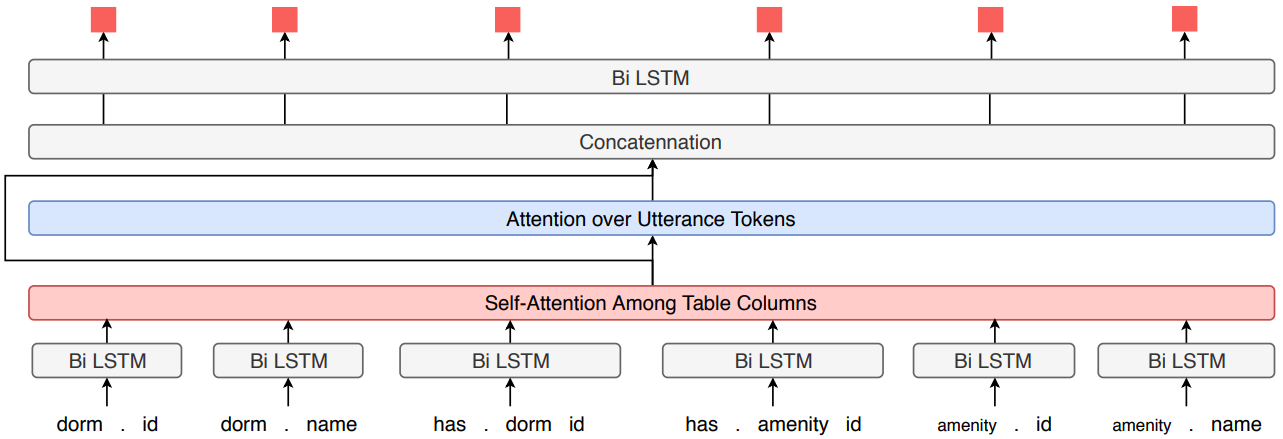
\includegraphics[width=0.8\textwidth]{pics/EditSQL/Table.png}
    \caption{The model architecture of EditSQL \cite{DBLP:journals/corr/abs-1909-00786}}
    \label{fig:EditSQL}
\end{figure}

User utterances and table schemas are encoded by the utterance-table encoder. Tokens of utterances are encoded using a bi-LSTM.
To determine the most relevant columns, Attention weighed an average of column header embedding is applied to each token.

\begin{figure}[H]
    \centering
    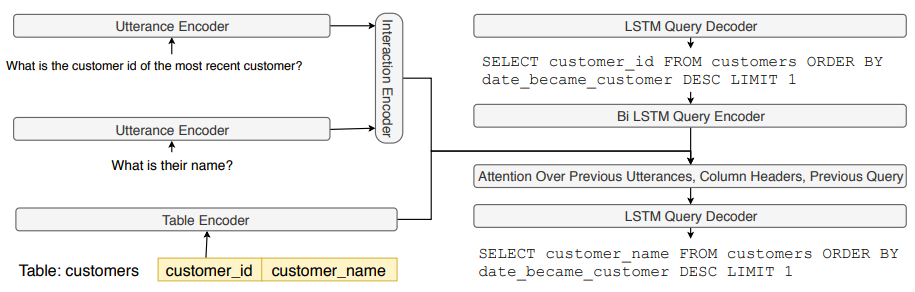
\includegraphics[width=0.9\textwidth]{pics/EditSQL/model.png}
    \caption{An example of user utterance and column headers and Utterance Encoder \cite{DBLP:journals/corr/abs-1909-00786}}
    \label{fig:EditSQL_model}
\end{figure}

To capture the relationship between table schema and utterance, an attention layer is incorporated.
The utterance-level encoder is built on top of an interaction-level decoder in order to capture information across utterances.
LSTM decoding is used to generate SQL queries by incorporating interaction history, table schema, and user utterances.

\begin{figure}[H]
    \centering
    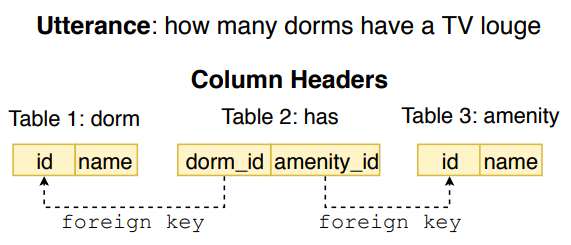
\includegraphics[width=0.5\textwidth]{pics/EditSQL/example.png}
    \caption{Table Encoder \cite{DBLP:journals/corr/abs-1909-00786}}
    \label{fig:EditSQL_example}
\end{figure}

The SPIDER dataset was used to evaluate the model, which outperformed the previous state-of-the-art model, such as IRNet. The model achieved a 32.9\% accuracy, and by using BERT embedding, a 57.9\% improvement in accuracy was achieved.